\section{Un Réseau}
\paragraph{Références} \cite{DarkWeb0}

\paragraph{Réseaux naturels, noeuds, liens}

\paragraph{} Bien que le terme de réseau ne s'utilise largement que depuis quelques dizaines d'années, il tire ses
racines plus anciennes du latin \emph{resel} qui signifiait \emph{le filet}. On retrouve ici la caractéristique
principale du réseau : ce sont des \emph{noeuds liés} entre eux selon un \emph{schéma}. Les réseaux existent en
premier lieu sous forme naturelle, on pense alors aux cours d'eau et à leur conjonctions, aux mouvements de troupeaux,
aux racines des arbres. Nous remarquons que les constructions humaines suivent également des réseaux : le réseau routier
avec les villes comme noeuds, le réseau ferré et les gares, le réseau électriques et les centrales..

\paragraph{} Toute création regroupant des noeuds avec des relations entre ces noeuds peut être qualifiée de "Réseau". En sciences,
la discipline qui s'occupe d'étudier les réseaux, et qui regroupe mathématique et informatique, s'appelle
la \emph{Théorie des Graphes}. Lorsque toute relation entre deux noeuds d'un graphe est symétrique, c'est à dire qu'elle va
dans un sens et dans l'autre, nous parlons de graphes \emph{non orientés}. Ce n'est par exemple pas le cas pour le
réseau routier qui est un graphe \emph{orienté}, car il possède des rues \emph{à sens unique}.

\begin{figure}[h]
    \centering
    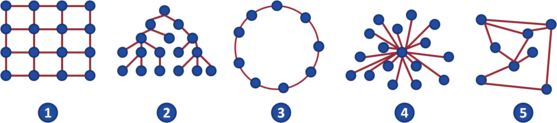
\includegraphics[width=400px]{chapters/02/images/reseaux.png}
    \caption{\label{Réseaux, graphes} Différentes formes de graphes}
\end{figure}

\paragraph{} On peut retrouver naturellement certaines de ces constructions. Le réseau hiérarchique (2) existe
au sein des sociétés, des gouvernements et des groupes d'Hommes en général. Il décrit généralement une structure
de contrôle par le haut, où le noeud le plus haut est dit parent des noeuds juste en dessous, et ainsi de suite.
Ainsi le pouvoir se concentre sur le haut du noeud et peut facilement être transmis verticalement, mais pas de 
manière transvese.

\paragraph{} On retrouve également le réseau centralisé (4) dans les organisations humaines par exemple,
où il traduit simplement la référence directe à un pouvoir supérieur. Les noeuds n'ont pas besoin de connaître
l'existence d'autres noeuds car ils se référent directement à une unité centrale qui sera \emph{décisionnaire}.
Souvent, les réseaux centralisés forment entre eux d'autres réseaux entralisés plus importants afin de reléguer
toute les \emph{micro-décisions} à une entité centrale supérieure qui sera en charge à partir de ces informations
de calculer une \emph{macro-décision}. On retrouve ici la notion de \emph{couches}, qui nous servira dans l'étude
de réseaux plus complexes.

\paragraph{Topologie réseau}

\paragraph{Réseau \emph{nominal}} "Idéal" de la mise en place d'un Réseau universel, omniprésent
et omniscient. Un tel système global impliquerait la mise en place d'un système hautement
distribué, voire \emph{"participatif"}.

\paragraph{Réseaux parallèles} Verra-t-on un jour la disparition des réseaux parallèles
(TOR, blockchains, ...) ? Ces technologies \emph{disruptives} seront-elles un jour vouées
à disparaitre ou au contraire à se développer avec d'autant plus d'ardeur ? Peut-on alors
parler d'une neutralisation du Réseau par le réseau ?

\paragraph{Objectif} L'objectif ici est de mettre en place un prototype qui se chargera de la récolte des données
de manière insidieuse et de leur mise ne réseau. Un logiciel, installé sur un ou plusieurs pc,
pourra envoyer des données à une entité centrale ou bien échanger entre eux.
